% !TeX program = xelatex

% CueTrace 台球厅销售推广手册 (Beamer)

% 编译：xelatex CueTrace.tex

\documentclass[aspectratio=169,11pt]{ctexbeamer}



\usepackage{tikz}

\usetikzlibrary{patterns,shadings,calc}

\usepackage{graphicx}

\usepackage{fontawesome5}



%==================== 品牌色 ====================

\definecolor{dachuan}{RGB}{6,126,249}      % 大川蓝

\definecolor{dachuanlt}{RGB}{96,170,255}   % 浅大川蓝

\definecolor{bgdark}{RGB}{6,8,12}          % 近黑底

\definecolor{bgmid}{RGB}{20,26,36}         % 质感高光灰

\definecolor{cardbg}{RGB}{16,20,28}

\definecolor{txtmain}{RGB}{236,240,246}

\definecolor{txtsub}{RGB}{150,160,175}



%==================== 主题外观 ====================

\usetheme{default}

\setbeamertemplate{navigation symbols}{}

\setbeamercolor{normal text}{fg=txtmain,bg=bgdark}

\setbeamercolor{frametitle}{fg=txtmain}

\setbeamercolor{itemize item}{fg=dachuan}

\setbeamercolor{itemize subitem}{fg=dachuanlt}

\setbeamercolor{structure}{fg=dachuan}

\setbeamerfont{frametitle}{size=\LARGE,series=\bfseries}

\setbeamertemplate{itemize item}{\textcolor{dachuan}{\faAngleRight}}

\setbeamertemplate{itemize subitem}{\textcolor{dachuanlt}{\scriptsize\faCircle}}



%==================== 有质感的黑色背景 ====================

\setbeamertemplate{background}{%

  \begin{tikzpicture}

    \useasboundingbox (0,0) rectangle (\paperwidth,\paperheight);

    % 基底纯黑

    \fill[bgdark] (0,0) rectangle (\paperwidth,\paperheight);

    % 左上径向高光，营造质感

    \shade[shading=radial,inner color=bgmid,outer color=bgdark]

      (0.30\paperwidth,0.78\paperheight) circle (0.95\paperwidth);

    % 细密点阵纹理

    \begin{scope}

      \clip (0,0) rectangle (\paperwidth,\paperheight);

      \foreach \x in {0,0.45,...,16.5}{

        \foreach \y in {0,0.45,...,9.5}{

          \fill[dachuan,opacity=0.05] (\x,\y) circle (0.012);

        }}

    \end{scope}

    % 斜向大川蓝光线

    \draw[dachuan,opacity=0.16,line width=1.1pt]

      (0.62\paperwidth,0) -- (\paperwidth,0.55\paperheight);

    \draw[dachuanlt,opacity=0.10,line width=0.6pt]

      (0.74\paperwidth,0) -- (\paperwidth,0.42\paperheight);

    \draw[dachuan,opacity=0.12,line width=0.8pt]

      (0,0.86\paperheight) -- (0.34\paperwidth,\paperheight);

  \end{tikzpicture}%

}



%==================== 帧标题：左侧蓝条 + 下划蓝线 ====================

\setbeamertemplate{frametitle}{%

  \vspace{0.55em}%

  \hspace{0.2em}%

  \begin{tikzpicture}

    \node[anchor=west,inner sep=0pt] (t) at (0,0)

      {\hspace{0.35em}\usebeamerfont{frametitle}\insertframetitle};

    \fill[dachuan] (-0.05,-0.42) rectangle (0.12,0.55);

    \draw[dachuan,opacity=0.55,line width=1.2pt]

      (-0.05,-0.62) -- ($(t.east)+(0.6,-0.62)$);

  \end{tikzpicture}%

  \vspace{0.2em}%

}



%==================== 页脚 ====================

\setbeamertemplate{footline}{%

  \hbox{}\vspace{2pt}%

  \hspace{0.6cm}%

  {\color{txtsub}\scriptsize CueTrace · 大川激流}\hfill

  {\color{dachuan}\scriptsize\faSquare}~{\color{txtsub}\scriptsize 台球训练数据智能管理系统}\hspace{0.4cm}%

  {\color{txtsub}\scriptsize\insertframenumber/\inserttotalframenumber}\hspace{0.6cm}%

  \vspace{6pt}%

}



%==================== 小工具命令 ====================

% 数据高亮块

\newcommand{\statbox}[2]{%

  \begin{tikzpicture}

    \node[draw=dachuan,line width=0.8pt,rounded corners=3pt,fill=cardbg,

      inner sep=8pt,text width=2.9cm,align=center] {%

      {\color{dachuanlt}\Large\bfseries #1}\\[2pt]

      {\color{txtsub}\scriptsize #2}};

  \end{tikzpicture}}



% 端能力卡片标题

\newcommand{\modtitle}[2]{{\color{dachuan}#1}\ {\bfseries\large #2}}



%==================== 界面还原（手机原型）配色与样式 ====================

\definecolor{screenbg}{RGB}{244,246,248}   % 小程序页面底色

\definecolor{uitext}{RGB}{31,35,41}         % UI 主文字

\definecolor{uiweak}{RGB}{138,144,153}      % UI 次文字

\definecolor{emptyc}{RGB}{235,237,240}      % 热力图空格

\definecolor{chipbg}{RGB}{225,239,255}      % 浅蓝标签底

\definecolor{thumbbg}{RGB}{234,242,255}     % 证书缩略底

\tikzset{

  bezel/.style={rounded corners=15pt, fill=black!90, draw=dachuan, line width=1pt, draw opacity=0.45},

  scr/.style={rounded corners=11pt, fill=screenbg},

  uicard/.style={rounded corners=6pt, fill=white},

  herocard/.style={rounded corners=6pt, fill=dachuan},

}



% persona 头像：把生成的人物图裁成圆形头像  #1文件 #2图宽 #3x偏移 #4y偏移 #5半径

\newcommand{\personaface}[5]{%

  \begin{tikzpicture}

    \begin{scope}

      \clip (0,0) circle (#5);

      \node[anchor=center,inner sep=0pt] at (#3,#4) {\includegraphics[width=#2]{#1}};

    \end{scope}

    \draw[dachuan,line width=1.4pt] (0,0) circle (#5);

  \end{tikzpicture}}



% 顶部状态栏（三端复用）

\newcommand{\uistatusbar}{%

  \node[anchor=west,uiweak,font=\tiny] at (0.45,7.96) {9:41};

  \node[anchor=east,uiweak,font=\tiny] at (3.78,7.96) {\faWifi~\faBatteryFull};}



%==================== 会员端界面：打卡热力图 ====================

\newcommand{\phonemember}{%

\resizebox{!}{0.74\paperheight}{%

\begin{tikzpicture}[x=1cm,y=1cm]

  \draw[bezel] (0,0) rectangle (4.2,8.4);

  \fill[scr] (0.16,0.16) rectangle (4.04,8.24);

  \uistatusbar

  % Hero

  \fill[herocard] (0.3,5.95) rectangle (3.9,7.7);

  \node[anchor=north west,white,font=\small\bfseries] at (0.5,7.55) {大川激流 · 训练打卡};

  \node[anchor=north west,white,opacity=0.85,font=\tiny] at (0.5,7.16) {坚持训练，点亮每一天的大川蓝};

  \foreach \x/\n/\l in {0.95/128/累计打卡天, 2.1/642/累计时长(h), 3.25/15/连续打卡天}{

    \node[anchor=north,white,font=\large\bfseries] at (\x,6.85) {\n};

    \node[anchor=north,white,opacity=0.85,font=\tiny] at (\x,6.4) {\l};}

  % 热力图卡

  \fill[uicard] (0.3,3.5) rectangle (3.9,5.8);

  \node[anchor=north west,uitext,font=\scriptsize\bfseries] at (0.5,5.66) {训练热力图};

  \node[anchor=north west,uiweak,font=\tiny] at (0.5,5.32) {近一年 · 单日越长颜色越深};

  \node[anchor=east,uiweak,font=\tiny] at (2.55,5.55) {少};

  \foreach \i in {0,1,2,3}{

    \pgfmathsetmacro{\op}{0.25+0.25*\i}

    \ifnum\i=0 \fill[emptyc] ({2.62+\i*0.18},5.48) rectangle ++(0.14,0.14);

    \else \fill[dachuan,opacity=\op] ({2.62+\i*0.18},5.48) rectangle ++(0.14,0.14);\fi}

  \node[anchor=west,uiweak,font=\tiny] at (3.42,5.55) {多};

  \foreach \c in {0,...,16}{

    \foreach \r in {0,...,6}{

      \pgfmathtruncatemacro{\m}{mod(\c*7+\r*11+\c,5)}

      \pgfmathtruncatemacro{\lv}{max(0,\m-1)}

      \pgfmathsetmacro{\px}{0.5+\c*0.19}

      \pgfmathsetmacro{\py}{4.95-\r*0.19}

      \ifcase\lv

        \fill[emptyc,rounded corners=0.4pt] (\px,\py) rectangle ++(0.15,0.15)%

      \or \fill[dachuan,opacity=0.35,rounded corners=0.4pt] (\px,\py) rectangle ++(0.15,0.15)%

      \or \fill[dachuan,opacity=0.65,rounded corners=0.4pt] (\px,\py) rectangle ++(0.15,0.15)%

      \else \fill[dachuan,rounded corners=0.4pt] (\px,\py) rectangle ++(0.15,0.15)%

      \fi;}}

  % 明细卡

  \fill[uicard] (0.3,1.3) rectangle (3.9,3.35);

  \node[anchor=north west,uitext,font=\scriptsize\bfseries] at (0.5,3.2) {今日训练明细};

  \node[anchor=north east,dachuan,font=\tiny] at (3.7,3.17) {总时长 3 小时 20 分};

  \fill[dachuan] (0.6,2.72) circle (0.05);

  \node[anchor=west,uitext,font=\tiny] at (0.74,2.8) {星河台球俱乐部};

  \node[anchor=west,uiweak,font=\tiny] at (0.74,2.52) {19:30 开始};

  \node[anchor=east,uitext,font=\tiny] at (3.7,2.68) {\bfseries 2 小时};

  \draw[black!8,line width=0.4pt] (0.5,2.28) -- (3.7,2.28);

  \fill[dachuan] (0.6,1.96) circle (0.05);

  \node[anchor=west,uitext,font=\tiny] at (0.74,2.04) {大川激流 · 旗舰店};

  \node[anchor=west,uiweak,font=\tiny] at (0.74,1.76) {21:00 开始};

  \node[anchor=east,uitext,font=\tiny] at (3.7,1.92) {\bfseries 1 小时 20 分};

  % 按钮

  \fill[herocard] (0.7,0.55) rectangle (3.5,1.12);

  \node[white,font=\scriptsize\bfseries] at (2.1,0.835) {+ 记录今日训练};

\end{tikzpicture}}}



%==================== 教练端界面：资料认证 ====================

\newcommand{\phonecoach}{%

\resizebox{!}{0.74\paperheight}{%

\begin{tikzpicture}[x=1cm,y=1cm]

  \draw[bezel] (0,0) rectangle (4.2,8.4);

  \fill[scr] (0.16,0.16) rectangle (4.04,8.24);

  \uistatusbar

  % 资料卡

  \fill[uicard] (0.3,5.25) rectangle (3.9,7.75);

  \begin{scope}

    \clip (0.95,6.95) circle (0.46);

    \node[anchor=center,inner sep=0pt] at (0.34,6.3) {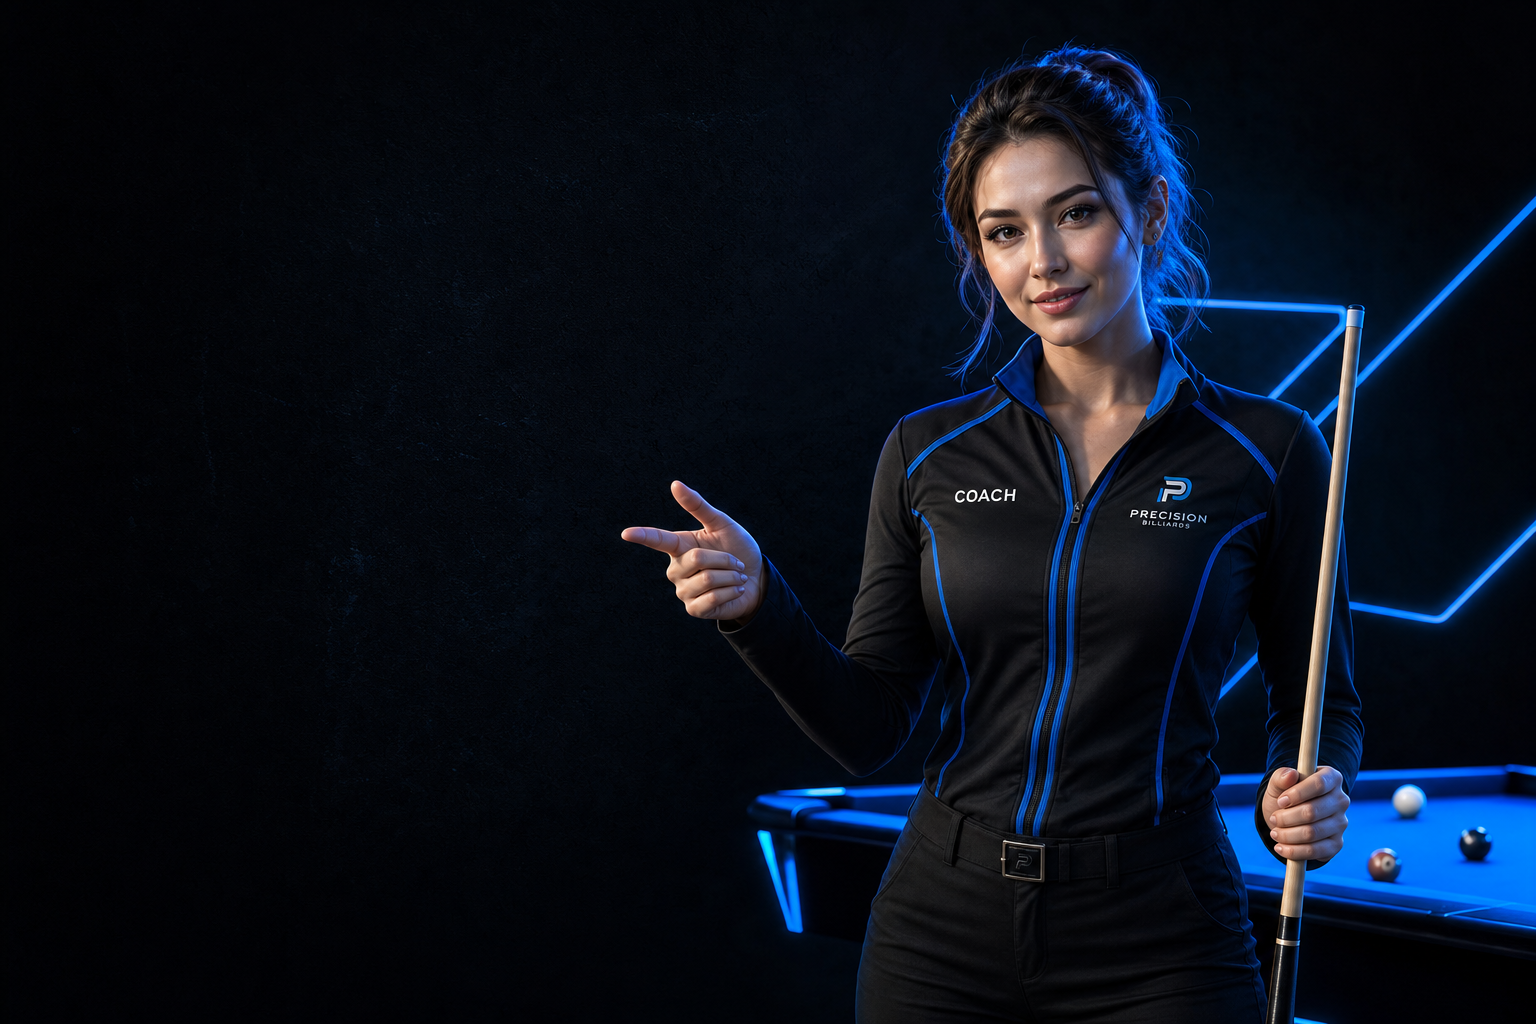
\includegraphics[width=3.3cm]{coach_female.png}};

  \end{scope}

  \draw[dachuan,line width=1pt] (0.95,6.95) circle (0.46);

  \node[anchor=west,uitext,font=\small\bfseries] at (1.55,7.18) {林晚 教练};

  \node[anchor=west,dachuan,font=\tiny] at (1.55,6.82) {\faCheckCircle~认证教练 · 球龄 12 年};

  \node[anchor=west,uiweak,font=\tiny] at (1.55,6.5) {教龄 6 年};

  \draw[black!8,line width=0.4pt] (0.5,6.05) -- (3.7,6.05);

  \node[anchor=west,uiweak,font=\tiny] at (0.5,5.8) {收费标准};

  \node[anchor=east,uitext,font=\tiny\bfseries] at (3.7,5.8) {3 元 / 分钟};

  \node[anchor=west,uiweak,font=\tiny] at (0.5,5.52) {一句话介绍};

  \node[anchor=east,uitext,font=\tiny] at (3.7,5.52) {职业级走位教学};

  % 证书卡

  \fill[uicard] (0.3,3.55) rectangle (3.9,5.05);

  \node[anchor=north west,uitext,font=\scriptsize\bfseries] at (0.5,4.9) {资格证书};

  \node[anchor=north east,uiweak,font=\tiny] at (3.7,4.9) {最多 6 张};

  \foreach \i in {0,1,2}{

    \pgfmathsetmacro{\tx}{0.5+\i*0.78}

    \fill[thumbbg,rounded corners=3pt] (\tx,3.75) rectangle ++(0.66,0.66);

    \node[dachuan,font=\small] at ({\tx+0.33},4.08) {\faCertificate};}

  \draw[dachuan,dashed,line width=0.6pt,rounded corners=3pt] (2.84,3.75) rectangle ++(0.66,0.66);

  \node[dachuan,font=\normalsize] at (3.17,4.08) {+};

  % 可约时段卡

  \fill[uicard] (0.3,1.45) rectangle (3.9,3.35);

  \node[anchor=north west,uitext,font=\scriptsize\bfseries] at (0.5,3.2) {可预约时段};

  \foreach \y/\t in {2.78/{周一 19:00 - 21:00}, 2.36/{周三 18:30 - 20:30}, 1.94/{周六 14:00 - 17:00}}{

    \fill[chipbg,rounded corners=4pt] (0.5,\y) rectangle ++(2.5,0.32);

    \node[anchor=west,dachuan,font=\tiny] at (0.62,{\y+0.16}) {\t};

    \node[anchor=east,uiweak,font=\tiny] at (3.7,{\y+0.16}) {删除};}

  % 按钮

  \fill[herocard] (0.7,0.55) rectangle (3.5,1.12);

  \node[white,font=\scriptsize\bfseries] at (2.1,0.835) {保存资料};

\end{tikzpicture}}}



%==================== 店家端界面：工作台 + 会员统计 ====================

\newcommand{\phoneshop}{%

\resizebox{!}{0.74\paperheight}{%

\begin{tikzpicture}[x=1cm,y=1cm]

  \draw[bezel] (0,0) rectangle (4.2,8.4);

  \fill[scr] (0.16,0.16) rectangle (4.04,8.24);

  \uistatusbar

  % Hero

  \fill[herocard] (0.3,5.95) rectangle (3.9,7.7);

  \node[anchor=north west,white,font=\small\bfseries] at (0.5,7.55) {大川激流 · 旗舰店};

  \node[anchor=north west,white,opacity=0.85,font=\tiny] at (0.5,7.16) {所属台球厅：星河台球俱乐部};

  \foreach \x/\n/\l in {0.95/8/在管教练, 2.1/126/本店会员, 3.25/3240/总训练(h)}{

    \node[anchor=north,white,font=\large\bfseries] at (\x,6.85) {\n};

    \node[anchor=north,white,opacity=0.85,font=\tiny] at (\x,6.4) {\l};}

  % 入口卡

  \fill[uicard] (0.3,4.2) rectangle (3.9,5.8);

  \foreach \y/\ic/\t/\s in {5.25/教/{教练名单}/{统一管理本店台球教练}, 4.55/会/{会员训练统计}/{查看打卡天数与训练时长}}{

    \fill[dachuan,rounded corners=4pt] (0.5,{\y-0.2}) rectangle ++(0.4,0.4);

    \node[white,font=\tiny\bfseries] at (0.7,\y) {\ic};

    \node[anchor=west,uitext,font=\tiny\bfseries] at (1.05,{\y+0.1}) {\t};

    \node[anchor=west,uiweak,font=\tiny] at (1.05,{\y-0.16}) {\s};

    \node[anchor=east,uiweak,font=\scriptsize] at (3.7,\y) {>};}

  \draw[black!8,line width=0.4pt] (0.5,4.9) -- (3.7,4.9);

  % 会员统计卡

  \fill[uicard] (0.3,1.3) rectangle (3.9,3.95);

  \node[anchor=north west,uitext,font=\scriptsize\bfseries] at (0.5,3.8) {会员训练统计};

  \node[anchor=west,uiweak,font=\tiny] at (0.5,3.4) {会员};

  \node[anchor=center,uiweak,font=\tiny] at (2.55,3.4) {打卡天数};

  \node[anchor=east,uiweak,font=\tiny] at (3.7,3.4) {训练时长};

  \foreach \y/\av/\nm/\d/\h in {2.95/王/{王浩}/96/642, 2.5/林/{林夕}/88/521, 2.05/陈/{陈默}/75/488, 1.6/赵/{赵岩}/63/402}{

    \fill[chipbg] (0.62,\y) circle (0.16);

    \node[dachuan,font=\tiny\bfseries] at (0.62,\y) {\av};

    \node[anchor=west,uitext,font=\tiny] at (0.88,\y) {\nm};

    \node[anchor=center,uitext,font=\tiny] at (2.55,\y) {\d 天};

    \node[anchor=east,dachuan,font=\tiny\bfseries] at (3.7,\y) {\h h};}

\end{tikzpicture}}}



\graphicspath{{assets/}{../assets/}}



%====================================================================

\begin{document}



%---------- 1. 封面 ----------

\begin{frame}[plain]

  \begin{tikzpicture}[overlay,remember picture]

    \node[anchor=center] at ($(current page.center)+(0,1.6)$)

      {\fontsize{52}{56}\selectfont\bfseries\color{txtmain}Cue\color{dachuan}Trace};

    \node[anchor=center] at ($(current page.center)+(0,0.2)$)

      {\Large\color{txtsub}大川激流 · 台球训练数据智能管理系统};

    % 分隔线

    \draw[dachuan,line width=1.4pt,opacity=0.8]

      ($(current page.center)+(-3.2,-0.5)$) -- ($(current page.center)+(3.2,-0.5)$);

    \node[anchor=center] at ($(current page.center)+(0,-1.3)$)

      {\color{txtmain}\large 让每一杆训练，都被看见};

    \node[anchor=center] at ($(current page.center)+(0,-2.1)$)

      {\color{txtsub}\small 会员端 · 教练端 · 店家端　|　品牌色 大川蓝 \#067EF9};

    \node[anchor=south east] at ($(current page.south east)+(-0.8,0.8)$)

      {\color{txtsub}\footnotesize 台球厅合作推广手册};

  \end{tikzpicture}

\end{frame}



%---------- 2. 行业痛点 ----------

\begin{frame}{台球厅，正在流失看不见的价值}

  \vspace{0.3em}

  \begin{columns}[T]

    \begin{column}{0.52\textwidth}

      \begin{itemize}

        \setlength{\itemsep}{0.85em}

        \item \textbf{会员留不住}：办卡即沉默，进步无感知，复购全凭人情

        \item \textbf{教练难量化}：教学水平、约课收费缺乏数据背书

        \item \textbf{经营靠拍脑袋}：到店、时长、活跃度没有沉淀，决策无依据

        \item \textbf{同质化竞争}：拼价格、拼位置，缺少差异化体验

      \end{itemize}

    \end{column}

    \begin{column}{0.46\textwidth}

      \vspace{0.6em}

      \begin{center}

        \statbox{60\%+}{新办卡会员\\3个月内不再活跃}\\[10pt]

        \statbox{凭感觉}{多数门店缺少\\会员训练数据}

      \end{center}

    \end{column}

  \end{columns}

  \vspace{0.6em}

  {\color{dachuanlt}\faLightbulb~\itshape 问题的本质：训练「看不见」，价值就「留不住」。}

\end{frame}



%---------- 3. 产品理念 ----------

\begin{frame}{CueTrace 理念：用数据让训练可见}

  \vspace{0.6em}

  \begin{center}

    {\Large\color{txtmain}把每一次到店训练，沉淀为\textbf{\color{dachuanlt}可视化的成长资产}}

  \end{center}

  \vspace{1.0em}

  \begin{columns}[T]

    \begin{column}{0.31\textwidth}

      \begin{center}

        {\color{dachuan}\Huge\faFingerprint}\\[8pt]

        \textbf{记录}\\[4pt]

        {\color{txtsub}\small 打卡热力图\\时长 · 频次 · 连续天数}

      \end{center}

    \end{column}

    \begin{column}{0.31\textwidth}

      \begin{center}

        {\color{dachuan}\Huge\faChartLine}\\[8pt]

        \textbf{量化}\\[4pt]

        {\color{txtsub}\small 教练资质 · 学员进步\\门店经营全景}

      \end{center}

    \end{column}

    \begin{column}{0.31\textwidth}

      \begin{center}

        {\color{dachuan}\Huge\faSync}\\[8pt]

        \textbf{留存}\\[4pt]

        {\color{txtsub}\small 看得见的进步\\驱动持续复购}

      \end{center}

    \end{column}

  \end{columns}

  \vspace{1.0em}

  \begin{center}

    \color{dachuanlt}\itshape 记录 → 量化 → 留存：一条把流量变留量的数据闭环。

  \end{center}

\end{frame}



%---------- 4. 产品架构总览 ----------

\begin{frame}{一套系统，三端协同}

  \vspace{0.4em}

  \begin{columns}[T]

    \begin{column}{0.32\textwidth}

      \begin{tikzpicture}

        \node[draw=dachuan,line width=1pt,rounded corners=5pt,fill=cardbg,

          inner sep=12pt,text width=3.5cm] {%

          \modtitle{\faUser}{会员端}\\[6pt]

          {\color{txtsub}\small GitHub 风格打卡热力图、训练明细、累计 / 连续天数}};

      \end{tikzpicture}

    \end{column}

    \begin{column}{0.32\textwidth}

      \begin{tikzpicture}

        \node[draw=dachuan,line width=1pt,rounded corners=5pt,fill=cardbg,

          inner sep=12pt,text width=3.5cm] {%

          \modtitle{\faChalkboardTeacher}{教练端}\\[6pt]

          {\color{txtsub}\small 资质认证、可约时段、收费标准、绑定学员看数据}};

      \end{tikzpicture}

    \end{column}

    \begin{column}{0.32\textwidth}

      \begin{tikzpicture}

        \node[draw=dachuan,line width=1pt,rounded corners=5pt,fill=cardbg,

          inner sep=12pt,text width=3.5cm] {%

          \modtitle{\faStore}{店家端}\\[6pt]

          {\color{txtsub}\small 教练统一管理、本店会员训练统计、经营概览}};

      \end{tikzpicture}

    \end{column}

  \end{columns}

  \vspace{1.0em}

  \begin{itemize}

    \setlength{\itemsep}{0.4em}

    \item \textbf{身份隔离}：会员 / 教练 / 店家三端工作台互不可见，权限清晰

    \item \textbf{微信小程序}：扫码即用，无需下载；云开发支撑，数据安全沉淀

  \end{itemize}

\end{frame}



%---------- 5. 会员端 · 界面与功能 ----------

\begin{frame}{会员端 · 界面与功能}

  \begin{columns}[T]

    \begin{column}{0.56\textwidth}

      \begin{flushright}\phonemember\end{flushright}

    \end{column}

    \begin{column}{0.44\textwidth}

      \begin{flushleft}

        \raisebox{-0.42cm}{\personaface{member_male.png}{3.2cm}{-0.55}{-0.66}{0.6}}\hspace{0.4em}%

        {\color{dachuanlt}\small 年轻球友\\的训练主场}

      \end{flushleft}

      \vspace{0.1em}

      \begin{itemize}

        \setlength{\itemsep}{0.28em}

        \item \textbf{打卡热力图}\\{\color{txtsub}\scriptsize 53 周 × 7 天网格，类 GitHub 贡献图}

        \item \textbf{时长分级点亮}\\{\color{txtsub}\scriptsize 0–3h / 3–8h / 8h+ 三档大川蓝深浅}

        \item \textbf{当日训练明细}\\{\color{txtsub}\scriptsize 点击格子看每家台球厅时长记录}

        \item \textbf{成长汇总}\\{\color{txtsub}\scriptsize 累计天数 · 累计时长 · 连续打卡}

      \end{itemize}

    \end{column}

  \end{columns}

\end{frame}



%---------- 6. 教练端 · 界面与功能 ----------

\begin{frame}{教练端 · 界面与功能}

  \begin{columns}[T]

    \begin{column}{0.44\textwidth}

      \begin{flushleft}

        \raisebox{-0.42cm}{\personaface{coach_female.png}{3.3cm}{-0.6}{-0.6}{0.6}}\hspace{0.4em}%

        {\color{dachuanlt}\small 专业教练\\的获客名片}

      \end{flushleft}

      \vspace{0.1em}

      \begin{itemize}

        \setlength{\itemsep}{0.28em}

        \item \textbf{资质认证}\\{\color{txtsub}\scriptsize 球龄 / 教龄 / 照片 / 资格证书多图}

        \item \textbf{透明收费}\\{\color{txtsub}\scriptsize X 元 / 分钟标准，约课更省心}

        \item \textbf{可约时段}\\{\color{txtsub}\scriptsize 按星期设置时段，灵活增删}

        \item \textbf{师生绑定}\\{\color{txtsub}\scriptsize 授权后只读看学员热力图与明细}

      \end{itemize}

    \end{column}

    \begin{column}{0.56\textwidth}

      \begin{flushleft}\phonecoach\end{flushleft}

    \end{column}

  \end{columns}

\end{frame}



%---------- 7. 店家端 · 界面与功能 ----------

\begin{frame}{店家端 · 界面与功能}

  \begin{columns}[T]

    \begin{column}{0.56\textwidth}

      \begin{flushright}\phoneshop\end{flushright}

    \end{column}

    \begin{column}{0.44\textwidth}

      \begin{flushleft}

        \raisebox{-0.28cm}{\begin{tikzpicture}

          \node[circle,draw=dachuan,line width=1.4pt,fill=cardbg,minimum size=1.0cm]

            {\color{dachuan}\large\faUsers};

        \end{tikzpicture}}\hspace{0.4em}%

        {\color{dachuanlt}\small 门店经营\\的数据驾驶舱}

      \end{flushleft}

      \vspace{0.1em}

      \begin{itemize}

        \setlength{\itemsep}{0.28em}

        \item \textbf{经营概览}\\{\color{txtsub}\scriptsize 在管教练 · 会员数 · 总训练时长}

        \item \textbf{教练名单}\\{\color{txtsub}\scriptsize 统一添加 / 移除、查看教练资料}

        \item \textbf{会员统计}\\{\color{txtsub}\scriptsize 打卡天数与时长，按时长降序排行}

        \item \textbf{数据资产}\\{\color{txtsub}\scriptsize 沉淀为门店专属的运营决策依据}

      \end{itemize}

    \end{column}

  \end{columns}

\end{frame}



%---------- 8. 价值主张 ----------

\begin{frame}{为什么台球厅需要 CueTrace}

  \vspace{0.4em}

  \begin{columns}[T]

    \begin{column}{0.48\textwidth}

      \modtitle{\faHeart}{留客复购}\par

      {\color{txtsub}\small 可视化进步形成「成长惯性」，热力图断签焦虑驱动持续到店。}

      \vspace{0.9em}\par

      \modtitle{\faTrophy}{差异化体验}\par

      {\color{txtsub}\small 「会用数据的台球厅」自带高端标签，提升品牌溢价。}

    \end{column}

    \begin{column}{0.48\textwidth}

      \modtitle{\faCoins}{教练增收}\par

      {\color{txtsub}\small 资质透明、约课便捷、数据背书，撬动私教课转化。}

      \vspace{0.9em}\par

      \modtitle{\faChartPie}{经营提效}\par

      {\color{txtsub}\small 用真实到店与时长数据做活动、做分层、做决策。}

    \end{column}

  \end{columns}

  \vspace{1.0em}

  \begin{center}

    \begin{tikzpicture}

      \node[draw=dachuan,line width=1pt,rounded corners=4pt,fill=cardbg,inner sep=9pt]

        {\color{txtmain}\small 零硬件改造 · 扫码即用 · 数据沉淀在门店自己手里};

    \end{tikzpicture}

  \end{center}

\end{frame}



%---------- 9. 合作落地方案 ----------

\begin{frame}{合作落地：轻量、快速、可见效}

  \vspace{0.5em}

  \begin{columns}[T]

    \begin{column}{0.33\textwidth}

      \begin{center}

        {\color{dachuan}\huge\faRocket}\\[6pt]\textbf{第 1 周 · 接入}\\[4pt]

        {\color{txtsub}\small 门店与教练资料录入\\小程序上线、码牌投放}

      \end{center}

    \end{column}

    \begin{column}{0.33\textwidth}

      \begin{center}

        {\color{dachuan}\huge\faUsers}\\[6pt]\textbf{第 2–4 周 · 激活}\\[4pt]

        {\color{txtsub}\small 会员打卡、教练约课\\首批训练数据沉淀}

      \end{center}

    \end{column}

    \begin{column}{0.33\textwidth}

      \begin{center}

        {\color{dachuan}\huge\faChartLine}\\[6pt]\textbf{第 2 月起 · 增长}\\[4pt]

        {\color{txtsub}\small 数据分层运营\\复购与私教转化提升}

      \end{center}

    \end{column}

  \end{columns}

  \vspace{1.1em}

  \begin{itemize}

    \setlength{\itemsep}{0.4em}

    \item \textbf{试点合作}：免费试用期内完成数据闭环验证，效果可量化

    \item \textbf{按店定制}：支持门店品牌、台球厅列表与收费规则灵活配置

  \end{itemize}

\end{frame}



%---------- 10. 路线图 + CTA ----------

\begin{frame}[plain]

  \begin{tikzpicture}[overlay,remember picture]

    \node[anchor=north west] at ($(current page.north west)+(0.9,-0.9)$)

      {\usebeamerfont{frametitle}\bfseries\color{txtmain}从打卡到\color{dachuan}智能训练};

  \end{tikzpicture}

  \vspace{2.0em}

  \begin{itemize}

    \setlength{\itemsep}{0.55em}

    \item \faCheckCircle~\textbf{里程碑 1–3}（已上线）：会员端 · 教练端 · 店家端

    \item \faCircleNotch~\textbf{里程碑 4}：台球社区 —— 视频 / 图文发帖、动态流

    \item \faCircleNotch~\textbf{里程碑 5}：摄像头单人训练 / 双人 PK 数据采集与分析

  \end{itemize}

  \vspace{1.4em}

  \begin{center}

    \begin{tikzpicture}

      \node[draw=dachuan,line width=1.2pt,rounded corners=5pt,fill=cardbg,inner sep=12pt]

        {\color{txtmain}\large 让我们一起，把您的台球厅升级为\ \color{dachuanlt}\textbf{数据驱动的训练空间}};

    \end{tikzpicture}\\[12pt]

    {\color{txtsub} CueTrace · 大川激流　|　欢迎预约现场演示与试点合作}

  \end{center}

\end{frame}



\end{document}

